\documentclass{article}

\usepackage{times,fullpage,graphicx,amsmath, subfigure}
\usepackage[pdfborder={0 0 0}]{hyperref}

\title{Methpipe Manual}

\begin{document}
\maketitle
The methpipe software package is a comprehensive tool chain for
analyzing whole genome bisulfite sequencing data (BS-Seq).  This
documentation will guide you step by step to learn how to perform the
data analysis in a BS-Seq project with methpipe. To facilitate
understanding of the work flow, we divide the analysis procedure into
four steps: (1) Pre-mapping processing: this step include assessing
read quality and pre-processing reads, such as trimming adapters; (2)
Mapping: this step maps sequence reads to a reference genome; (3)
Analyzing methylation status at single site: in this step, we will
estimate methylation frequency at single site, either CpG sites or
non-CpG sites. We will also obtain information about sequencing depth
and bisulfite conversion rate; (4) Higher level analysis: this step
includes higher level more biologically interesting analysis, such as
identifying hypo-methylated regions and/or differentially methylated
regions. Later we will describe in detail the usage of tools in each
step.

In the guide we will use a small project as example. Suppose that in
this project you would like to study the methylation pattern in two
cell types, B cells and neutrophiles. The B cell methylome is profiled
with sing-end sequencing and your university's sequencing center sends
back to you these sequence files:
\begin{verbatim}
bcell/s-1.fq bcell/s-2.fq bcell/s-3.fq bcell/s-4.fq.
\end{verbatim}
The neutrophile methylome is profiled with pair-end sequencing and you
have the following sequences files:
\begin{verbatim}
neut/s-1-1.fq neut/s-1-2.fq neut/s-2-1.fq neut/s-2-2.fq.
\end{verbatim}
Now we are ready to uncover the interesting biology about DNA
methylation from this dataset. 

\section{Pre-mapping processing}
\label{sec:premapping}
% \begin{description}
% \item[read-quality-prof.cpp]
% This program take a fastq file as input and output the base composition and 
% quality scores for each column
% \item[quality-prof.R]
% This R script define a function that takes the output of read-quality-prof.cpp as input 
% and draw the figure of base composition
% \item[trim-adapter.cpp] 
% This program expects a fastq file as input and trim the adapter sequence from the 3' end
% of reads if there is.
% \item[visireads.cpp]
% This program takes a fastq file as input and output a BED file displaying Cs in 
% the sequences
% \end{description}

Before mapping sequenced reads to a reference genome, we need to
pre-process the raw read sequences, in particular we need to trim
possible adapter sequences retained in the 3' end of raw
reads. Further we may be interested in examining the quality of reads
in our library and visualizing raw reads in UCSC Genome Browser. 

\subsection{Trim adapters}
\label{sec:trim-adapter}
As the length of reads that sequencing technology is able to produce
has been increasing all the time, it is possible there are adapter
sequences in the 3' end of some reads. These retained adapter
sequences affects the mappability of such reads. Even if they are
somehow mapped to the reference genome, the adapter sequences may
introduce bias to our estimate of methylation frequency. Therefore it
is necessary to trim these retained adapter sequences. 

The program \textbf{trim-adapter} is used to trim adapter sequences,
if any, from the 3' end of raw reads. Suppose the adapter sequences is
\textit{GATCGGAAGAGCGGTTCAGCAGGAATGCCGAGACCGATCTCGTATGCCG}, we trim
the adapter sequences from raw reads in the file bcell/s-1.fq with the
following command:
\begin{verbatim}
$ ./trim-adapter  s-1.fq -o s-1-clipped.fq  
-a GATCGGAAGAGCGGTTCAGCAGGAATGCCGAGACCGATCTCGTATGCCG  
\end{verbatim}

If you would like to check the effective read length after trimming
adapter sequences and Ns from 3' end, you can add \textbf{-l} options
to specify the output file for effective read length, for example,
\begin{verbatim}
$ ./trim-adapter  s-1.fq -o s-1-clipped.fq  -l s-1-length.txt
-a GATCGGAAGAGCGGTTCAGCAGGAATGCCGAGACCGATCTCGTATGCCG  
\end{verbatim}
The file s-1-length.txt lists the effective read length of each read
after trimming adapter sequences and Ns, which can be used to compute
the statistics of effective reads lengths with any general purpose
statistical package, such as R. Perform this trimming adapter
processing on all sequences files and for convenience we assume the
processed sequences files have their original file names thereafter.

\subsection{Assessing read quality}
\label{sec:read-qual-assessm}
It is optional to assess read quality before mapping, however such
assessment may help us to spot potential problems during library
preparation and/or bisulfite sequencing. The program
\textbf{read-quality-prof} is used to generate an average summary of
base composition and quality scores from 5' to 3' along all
reads.  We run \textbf{read-quality-prof} as following 
\begin{verbatim}
$ ./read-quality-prof  < s-1.fq > s-1-qual.txt
\end{verbatim}
The output file s-1-qual.txt can be visualized with the R software. 
Fig. \ref{fig:base-composition} shows the base composition profile in
the pair-end sequencing sample, where the left panel shows  T-rich
reads and the right panel A-rich reads. Note the small proportion of C
and G reflects the effect of bisulfite conversion.   

\begin{figure}[htbp]
  \centering
\subfigure[T-rich reads]{
  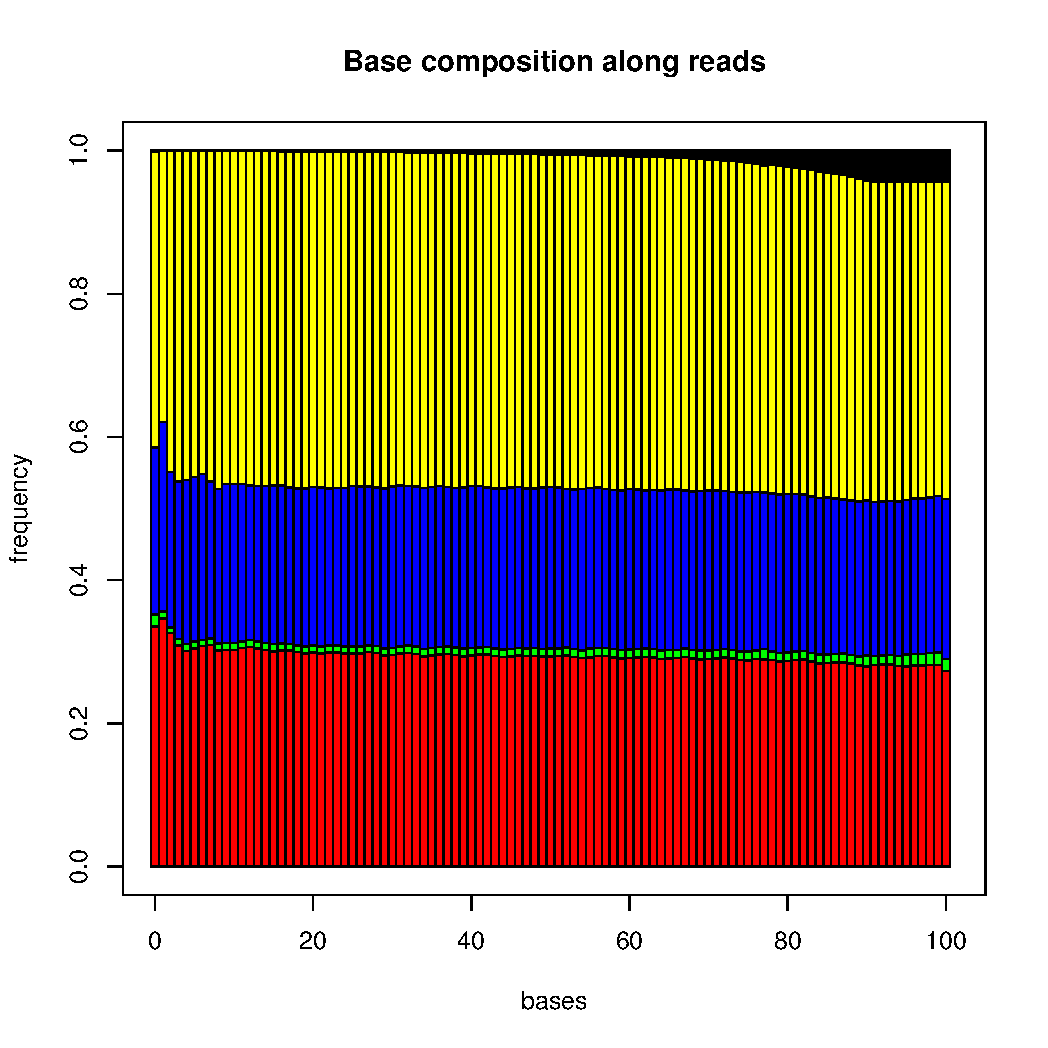
\includegraphics[width=2.8in]{figs/T-rich-base-composition.pdf}
}
\subfigure[A-rich reads]{
  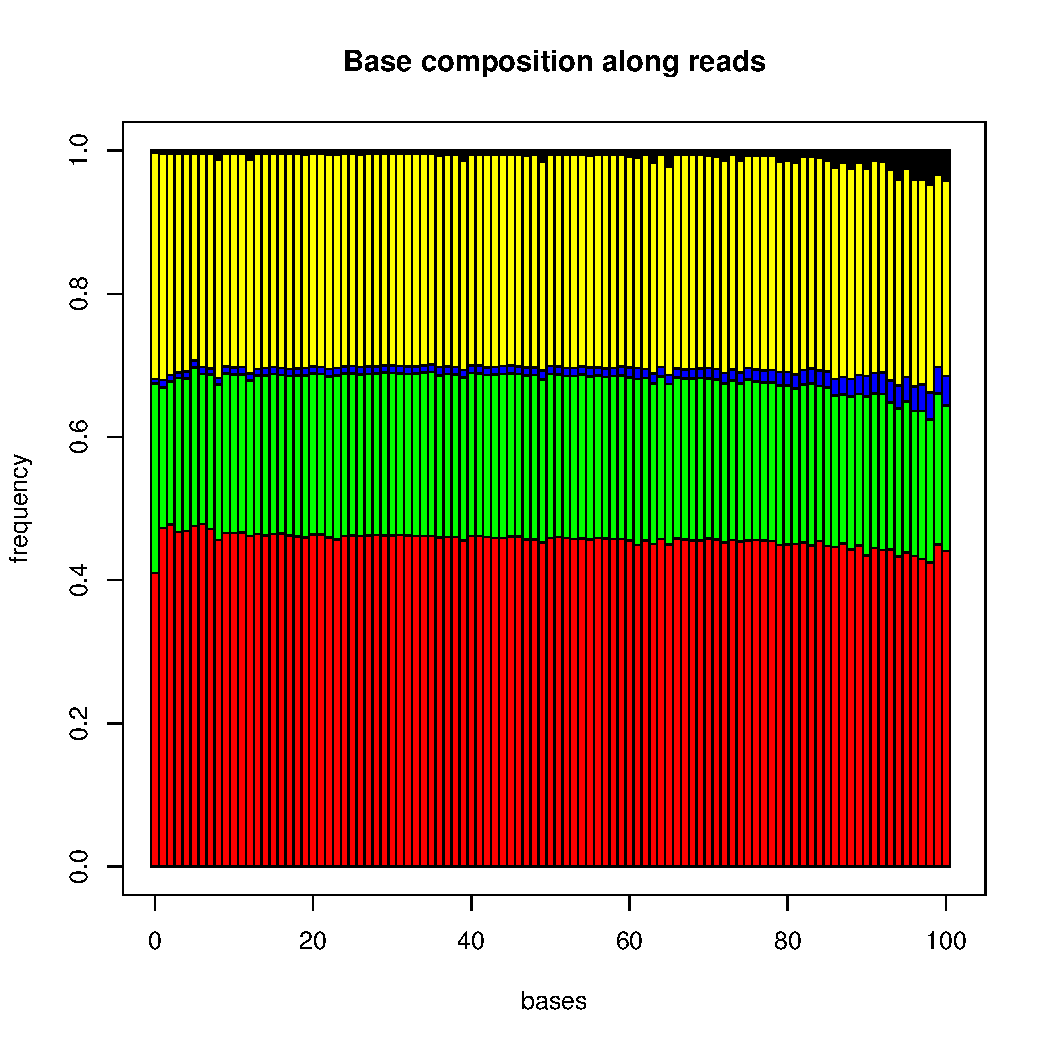
\includegraphics[width=2.8in]{figs/A-rich-base-composition.pdf}
}
  \caption{Base composition}
  \label{fig:base-composition}
\end{figure}


\section{Mapping}
\label{sec:mapping}

% \begin{description}
% \item[rmapbs.cpp]
% This program takes fastq file as input and output mapped read file
% \end{description}

In the mapping step, you will map sequence reads to a reference
genome. During bisulfite treatment, unmethylated cytosines in the
original DNA sequences are converted to uracils, which are in turn
incorporated as thymines during PCR amplification. We call such strand
T-rich and its complementary strand A-rich (adenine-rich).  When
mapping T-rich reads to the reference genome, either a cytosine (C) or
a thymine (T) in reads is considered valid match to a cytosine in the
reference genome. But for A-rich reads, a adenine or a guanine is
consider valid match to a guanine in the reference genome.    

If using single-end sequencing, you will get T-rich reads only. If
using pair-end sequencing, you will get both T-rich reads and A-rich
reads. Next we will learn how to map bisulfite treated reads with
\textbf{rmapbs} from either single-end sequencing or pair-end
sequencing. 

\subsection{Mapping single-end sequencing reads}
\label{sec:mapping-single-end}
Mapping read sequences to the reference genome is done by
\textbf{rmapbs}. Before mapping, you need to get he genome sequences
of appropriate organism and assembly, which is usually downloadable
from \href{http://hgdownload.cse.ucsc.edu/downloads.html}{UCSC Genome
  Browser download portal} or other specific repositories of genome
sequences, such as \href{http://www.arabidopsis.org/}{TAIR} for
Arabidopsis \textit{thaliana}. Suppose that you have already
downloaded the appropriate genome sequences, in our example human
genome hg18, in the directory \textit{human-genome}, to map the reads
in bcell/s-1.fq to the reference genome we run
\begin{verbatim}
$ ./rmapbs -c human-genome -s fa -m 4 -o bcell/s-1.bed bcell/s-1.fq -v. 
\end{verbatim}
The option \textbf{-c} specifies the direcotory holding the reference
genome and the \textbf{-s} specifies the suffix of sequence file
names. The option \textbf{-m} gives the maximum number of mismatches
allowed. The option \textbf{-o} specifies the output file. There are
other options to fine tune the behavior of \textbf{rmapbs} which are
explained on methpipe website.  

\subsection{Mapping pair-end sequencing reads}
\label{sec:mapping-pair-end}
At present our pipeline map R-rich reads and A-rich reasd separately
when mapping reads from the pair-end sequencing procedure. We map
T-rich reads in the same way as for single end-reads. However we use
A/G wildcards when mapping the A-rich reads, i.e. a adenine or a
guanine is considered valid match to a guanine in the reference
genome. The \textbf{rmapbs}, given the option \textbf{-A}, run in A/G
wildcard mode. Therefore to map T-rich reads, for example,
neut/s-1-1.fq, we run
\begin{verbatim}
$ ./rmapbs -c human-genome -s fa -m 4 -o neut/s-1-1.bed neut/s-1-1.fq -v. 
\end{verbatim}
To map A-rich reads, for example neut/s-1-2.fq, we run 
\begin{verbatim}
$ ./rmapbs -c human-genome -s fa -m 4 -o neut/s-1-2.bed neut/s-1-2.fq -v -A. 
\end{verbatim}
The other options have the same meaning in both C/T wildcard mode and
A/G wildcard mode.   

\subsection{Parallel mapping}
\label{sec:parallel-mapping}
Mapping is the most time-consuming and resource-demanding step in the
methpipe pipeline. Fortunately we may adopt a ``divide and conquer''
strategy to speed up this step.  In brief, we first divide large
sequence files into smaller ones, map them separately in parallel and
finally combining the mapped files.

A large sequence file is divided into smaller ones with the
\textbf{split} utility which is a standard utility in any UNIX-like
platforms. By running
\begin{verbatim}
$ split -l 16000000 bcell/s-1.fq s-1
\end{verbatim}
you will get a series of smaller files: s-1aa, s-1ab, s-1ac, etc,
which can be mapped with \textbf{rmapbs} separately as described
above. To learn about the detailed usage of \textbf{split}, you may
read its man page. In brief, the \textbf{-l} option specifies the
number of lines in each smaller file. Since FASTQ format requires that
each read consist of four lines, i.e. name line, sequence line, name
line and score line, the number of lines should be multipliers of
4. The optimal number depends on the time constraints and memory
contraints of your computing platform. For your information, mapping
$28$ millions reads to the Arabidopsis \textit{thaliana} genome with
\textbf{rmapbs} uses about 40 minutes and 5Gb memory. 

\section{Post-mapping processing}
\label{sec:postmapping}

% \begin{description}
% \item[merge.cpp]
% merge sorted MappedRead file, with option to control whether remove redundant file

% \item[mask-overlap.cpp]
% mask overlapping region of paired-reads, also generate summary of fragment length,
% number of unpaired reads

% \item[unique.cpp ]
% filter program to remove duplicate reads

% \item[ sort.cpp ]
% sort MappedRead file: either by genomic location or by name

% \item[ revcomp.cpp ]
% do reverse complement operation on MappedRead

% \end{description}

If everything goes well, you should already have pre-processed raw
sequence reads and mapped them to the reference genome. Suppose the
mapped reads files of B cell sample are
\begin{verbatim}
bcell/s-1.bed bcell/s-2.bed bcell/s-3.bed bcell/s-4.bed,
\end{verbatim}
and the mapped reads files of the neutrophile sample methylome are
\begin{verbatim}
neut/s-1-1.bed neut/s-1-2.bed neut/s-2-1.bed neut/s-2-2.bed.
\end{verbatim}
We will discuss some necessary processing steps, including converting
A-rich reads to T-rich reads in pair-end sequencing, masking
overlapping regions of paired reads, handling duplicate reads and
utilities to sort and/or merge mapped reads. 

\subsection{Converting A-rich reads to T-rich reads}
\label{sec:conv-rich-reads}
As has been noted before, if using pair-end sequencing, you will get
both T-rich reads and A-rich reads. When estimating methylation
frequency of a cytosine residue, we count the number of cytosines,
which originate from methylated cytosines, and the number of thymines,
which originate from unmethylated cytosines, and the use the ratio
$\frac{\#C}{\#C+\#T}$ as the estimate of methylation frequency of that
base. Therefore, A-rich reads need to be converted to T-rich reads
before we are able to leverage the information from these A-rich
reads. This conversion is easily done with the program
\textbf{revcomp}, for example  
\begin{verbatim}
$ ./revcomp < neut/s-2-2.bed > neut/s-2-2-revcomp.bed
\end{verbatim}
Note this conversion applies to and only applies to A-rich reads in
pair-end sequencing. For notation convenience, we again assume you
rename the converted reads file name to its original file name
thereafter.

\subsection{Masking overlapping regions of paired reads}
\label{sec:mask-overl-regi}
With pair-end sequencing, we obtain two reads: a T-rich read from 3'
end of the orignal segments and an A-rich read from 5' end. After
converting A-rich read to T-rich read, we have two T-rich reads from
the orignal DNA segment, which possibly overlap for certain
proportion. This overlapped region, if left as-is, will result in bias
that cytosines (or thymines if unmethylated) from the same DNA
molecule are counted twice. 

The program \textbf{mask-overlap} identifies and masks overlapped
regions. In our example project, neut/s-1-1.bed and neut/s-1-2.bed
contain T-rich reads and A-rich reads (converted) respectively. We
first sort the reads in these two files by name by running
\begin{verbatim}
$ ./sort -N neut/s-1-1.bed -o tmpfile && mv tmpfile neut/s-1-1.bed
$ ./sort -N neut/s-1-2.bed -o tmpfile && mv tmpfile neut/s-1-2.bed,
\end{verbatim}
And then we run \textbf{mask-overlap} to mask overlapping regions of
reads from these two files
\begin{verbatim}
$ ./mask-overlap neut/s-1-1.bed neut/s-1-2.bed 
neut/s-1-1-masked.bed neut/s-1-2-masked.bed.
\end{verbatim}
Note the commandline argument to \textbf{mask-overlap} are
input-file-1, input-file-2, output-file-1 and output-file-2. 

The program \textbf{mask-overlap} can also be used to obtain the
following information about the pair-end sequencing data, such as the
DNA fragment length distribution and the number of unpaired reads
after mapping. This is done by specifying the fragment length file
with the \textbf{-f} option. For example,
\begin{verbatim}
$ ./mask-overlap -f neut/s-1-length.txt  neut/s-1-1.bed neut/s-1-2.bed 
neut/s-1-1-masked.bed neut/s-1-2-masked.bed.
\end{verbatim}
In the file neut/s-1-length.txt \textbf{mask-overlap} write the
fragment length based on each pair of reads. This file can then be
analyzed with statistical software and standard *NIX text-processing
utilities. 

\subsection{Sorting reads}
\label{sec:sorting-reads}
The \textbf{sort} utility is used to sort mapped reads according to
different criterion. The usage of \textbf{sort} is quite
straightforward. To sort reads according to their genomic locations,
we run
\begin{verbatim}
$ ./sort bcell/s-1.bed -o output-file.
\end{verbatim}
To sort reads according to their names we run 
\begin{verbatim}
$ ./sort -N bcell/s-1.bed -o output-file.
\end{verbatim}

\subsection{Merging read files}
\label{sec:merging-reads-files}
The final step before estimating methylation frequency and performing
other higher level analysis is to merge read files from different
sequencing lanes and/or flowcells. 

If all read files are generated from the same biological library, this
step is quite straightforward. We sort all read files by genomic
locations with \textbf{sort} (Section \ref{sec:sorting-reads}), merge
those files with \textbf{merge} and then remove duplicate reads with
\textbf{unique} (Section \ref{sec:proc-dupl-reads}). We show how to
merge read files in the B cell data below.
\begin{verbatim}
$ # sort read files
$ ./sort bcell/s-1.bed -o tmpfile && mv tmpfile bcell/s-1.bed
$ ./sort bcell/s-2.bed -o tmpfile && mv tmpfile bcell/s-2.bed
$ ./sort bcell/s-3.bed -o tmpfile && mv tmpfile bcell/s-3.bed
$ ./sort bcell/s-4.bed -o tmpfile && mv tmpfile bcell/s-4.bed
$ ./merge bcell/s-*bed |./unique > bcell/bcell.bed 
\end{verbatim}

If the read files are from different libraries, it takes some extra
step. The reason is that: even if two reads from different biological
libraries are mapped to the same location, they are not originated
from the same DNA molecule, therefore both should be kept for
downstream analysis. For each library, we pool reads from this library
and remove duplicate reads. Then we merge reads from different
libraries. 

\subsection{Removing duplicate reads}
\label{sec:proc-dupl-reads}
Because of PCR bias and other unknown causes, there are tens of
thousands of reads mapped to exactly the same location in some regions
of the genome while the average sequencing depth is usually below
20. These large amounts of reads are likely orginated from the same
DNA segments and will possibly bias the estimation of methylation
frequency. One approach to alleviate this bias, though not completely
justifiable, is to keep only one distint read at each starting
position. This task is done by the program unique \textbf{unique}. For
example if we would like to remove duplicate reads from the file
bcell/s-1.bed, we can run 
\begin{verbatim}
$ ./unique bcell/s-1.bed -o bcell/s-1-unique.bed
\end{verbatim}

\section{Methylation frequency and bisulfite conversion rate}
\label{sec:estim-methyl-freq}
% \begin{description}
% \item[methcount.cpp]
% This program reads mapped read file and output methylation frequency
% for each CpG site.
% \item[bsrate.cpp]
% This program reads mapped read file and estimate bisulfite conversion
% rate by checking methylation status of non-CpG C's
% \end{description}

\subsection{Estimating methylation frequency}
\label{sec:estim-methyl-freq}

\subsection{Estimating busilfite conversion rate}
\label{sec:estim-busilf-conv}

\section{Higher level analysis}
\label{sec:high-level-analys}

\subsection{Identifying hypo-methylated regions}
\label{sec:ident-hypo-methyl}

\subsection{Identifying differentially methylated regions}
\label{sec:ident-diff-methyl}


\section{Visualization}
\label{sec:visualization}





\section{A sample work flow}
This part shows how these tools are connected to get the methylation
profile. Suppose we have the following BS-Seq library
\begin{verbatim}
reads/s_1_1.txt reads/s_1_2.txt reads/s_2_1.txt reads/s_2_2.txt
\end{verbatim}

The final result can be obtained as following. For clarity, we show
all the intermediate result. In real application, some intermediate
files can be avoided by using pipes.

\begin{verbatim}
# Pre-mapping processing #

## trim adapter ##
$ ./trim-adapter reads/s_1_1.txt preprocessed/s_1_1.txt
$ ./trim-adapter reads/s_1_2.txt preprocessed/s_1_2.txt
$ ./trim-adapter reads/s_2_1.txt preprocessed/s_2_1.txt
$ ./trim-adapter reads/s_2_2.txt preprocessed/s_2_2.txt

# Mapping #
$ ./rmapbs -c genome_seq_dir -o mapped/s_1_1.mr preprocessed/s_1_1.txt
$ ./rmapbs -A -c genome_seq_dir -o mapped/s_1_2.mr preprocessed/s_1_2.txt
$ ./rmapbs -c genome_seq_dir -o mapped/s_2_1.mr preprocessed/s_2_1.txt
$ ./rmapbs -A -c genome_seq_dir -o mapped/s_2_2.mr preprocessed/s_2_2.txt

# post-mapping processing

## reverse complement A-rich strand ##
$ ./revcomp mapped/s_1_2.mr > tmpfile && mv tmpfile mapped/s_1_2.mr
$ ./revcomp mapped/s_2_2.mr > tmpfile && mv tmpfile mapped/s_2_2.mr

## mask overlapping ##
#### first sort by name ####
$ ./sort -N mapped/s_1_1.mr -o tmpfile && mv tmpfile  mapped/s_1_1.mr 
$ ./sort -N mapped/s_1_2.mr -o tmpfile && mv tmpfile  mapped/s_1_2.mr 
$ ./sort -N mapped/s_2_1.mr -o tmpfile && mv tmpfile  mapped/s_2_1.mr 
$ ./sort -N mapped/s_2_2.mr -o tmpfile && mv tmpfile  mapped/s_2_2.mr 

#### masking ####
$ ./mask-overlap mapped/s_1_1.mr mapped/s_1_2.mr masked/s_1_1.mr masked/s_1_2.mr
$ ./mask-overlap mapped/s_2_1.mr mapped/s_2_2.mr masked/s_2_1.mr masked/s_2_2.mr

#### sort by genomic location ####
$ ./sort masked/s_1_1.mr -o tmpfile && mv tmpfile  masked/s_1_1.mr 
$ ./sort masked/s_1_2.mr -o tmpfile && mv tmpfile  masked/s_1_2.mr 
$ ./sort masked/s_2_1.mr -o tmpfile && mv tmpfile  masked/s_2_1.mr 
$ ./sort masked/s_2_2.mr -o tmpfile && mv tmpfile  masked/s_2_2.mr 

## combine all result ##
#### merge ####
$ ./merge -o all.mr masked/s_1_1.mr masked/s_1_2.mr masked/s_2_1.mr masked/s_2_2.mr 

#### jackpot removal #####
$ ./unique all.mr -o tmpfile && mv tmpfile all.mr

# analysis #
## methcounts ##
$ ./methcounts -c genome_sequence_file -o all-methcounts.bed all.mr 
\end{verbatim}

\end{document}


